\documentclass{article}
\usepackage[T1]{fontenc}
\usepackage[francais]{babel}
\usepackage[utf8]{inputenc}

\usepackage{amsmath,amsfonts,amsthm} % Math packages
\usepackage[pdftex]{graphicx}
\usepackage{hyperref}
\usepackage{lipsum}

\usepackage{listings}
\usepackage{charter}
\usepackage{array}
\usepackage{here}
\usepackage[justification=centering,singlelinecheck=false]{caption}
\usepackage{subcaption}
\newcolumntype{M}[1]{>{\raggedright}m{#1}}
\newcommand{\HRule}{\rule{\linewidth}{0.5mm}}


%Listing Alloy
\lstdefinelanguage{alloy}{
  keywords={%
      assert, pred, all, no, lone, one, some, check, run,
      but, let, implies, not, iff, in, and, or, set, sig, Int, int,
      if, then, else, exactly, disj, fact, fun, module, abstract,
      extends, open, none, univ, iden, seq, enum
  },
  sensitive=true,  % case sensitive
  morecomment=[l]//,%
  morecomment=[l]{--},%
  morecomment=[s]{/*}{*/},%
  morestring=[b]",
  numbers=none,
  firstnumber=1,
  aboveskip=3mm,
  belowskip=3mm,
  frame=single,
  showstringspaces=false,
  numberstyle=\tiny,
  stepnumber=2,
  breaklines=true,
  breakatwhitespace=true,
  tabsize=3,
  basicstyle={\small\ttfamily},
  commentstyle=\itshape,
  columns=flexible,
  keywordstyle=\color{blue}\bfseries,
  ndkeywordstyle=\bfseries,
}

% inline
\def\A{%
    \lstinline[language=alloy,basicstyle=\ttfamily,columns=fixed]}
 
% paragraph
\lstnewenvironment{alloy}[1][]{%
  \lstset{language=alloy,
    floatplacement={tbp},captionpos=b,
    xrightmargin=8pt,basicstyle=\ttfamily,#1}}{}

%Listing Alloy in tab
\lstdefinelanguage{alloyt}{
  keywords={%
      assert, pred, all, no, lone, one, some, check, run,
      but, let, implies, not, iff, in, and, or, set, sig, Int, int,
      if, then, else, exactly, disj, fact, fun, module, abstract,
      extends, open, none, univ, iden, seq, enum
  },
  sensitive=true,  % case sensitive
  morecomment=[l]//,%
  morecomment=[l]{--},%
  morecomment=[s]{/*}{*/},%
  morestring=[b]",
  numbers=none,
  firstnumber=1,
  aboveskip=3mm,
  belowskip=3mm,
  showstringspaces=false,
  numberstyle=\tiny,
  stepnumber=2,
  breaklines=true,
  breakatwhitespace=true,
  tabsize=3,
  basicstyle={\small\ttfamily},
  commentstyle=\itshape,
  columns=flexible,
  keywordstyle=\color{blue}\bfseries,
  ndkeywordstyle=\bfseries,
}

% paragraph
\lstnewenvironment{alloyt}[1][]{%
  \lstset{language=alloyt,
    floatplacement={tbp},captionpos=b,
    xrightmargin=8pt,basicstyle=\ttfamily,#1}}{}
 

 
\usepackage{color}
\definecolor{dkgreen}{rgb}{0,0.6,0}
\definecolor{gray}{rgb}{0.5,0.5,0.5}
\definecolor{mauve}{rgb}{0.58,0,0.82}

\begin{document}

%\title{Génération et analyse automatisées d’ensembles de règles pour Picobot}
%\author{Quentin BAILLEUL \  Jérémy BOSSUT \  Romain PHILIPPON}


%\maketitle
\begin{titlepage}
\begin{center}

% Upper part of the page. The '~' is needed because \\
% only works if a paragraph has started.

\includegraphics[width=0.5\textwidth]{pictures/ul.png}~\\[1cm]

% Title
\HRule \\[0.2cm]
{ \huge \bfseries Simulation à base d'agents de l'évolution d'un
  logiciel Open Source \\[0.4cm] }

\HRule \\[1.5cm]
Quentin BAILLEUL \  Romain PHILIPPON

\vfill

% Bottom of the page
{\large \today}

\end{center}
\end{titlepage}

\newpage
\tableofcontents

\newpage

\section{Introduction}
%inspiration du abstract de base
L'informatique est une discipline qui évolue rapidement et
il est nécessaire de comprendre
les processus évolutifs qui prévalent dans de nouvelles formes de
développement de logiciels, surtout dans un environement Open source.
\\

Beaucoup de travaux et d'analyses sont fournies à propos de la
création et de l'évolution de logiciels propriétaires, à l'inverse de
l'étude sur les logiciels Open Sources. (?)Ceux-ci ayant un environement
et donc une évolution différente (?). 
\\

Ce qui suggère que les théories existantes sur l'évolution des logiciels
sont différentes pour les logiciels open source.

Dans cet optique les recherches de N Smith, A Capiluppi, et
J Fernandez-Ramil tendent(?) et améliorer voir redéfinir ces théories
\\

Leur article(mettre source) utilise les théories de l'évolution du logiciel
afin de reproduire et d'expliquer les observations empiriques d'un ensemble
de systèmes Open Source.

L'article se repose sur une simulation multi-agents de
développement logiciel dans un environement Open Source
\\

Le but de ce rapport sera de modifier la simulation en ajouter des
paramêtre afin de rajouter du réalisme (inverse du rasoir d'ocam) et
enfin de comparer les résultats.

\section{Simulation de base}
\subsection{Modèle}

\begin{figure}[H]
 \centerline{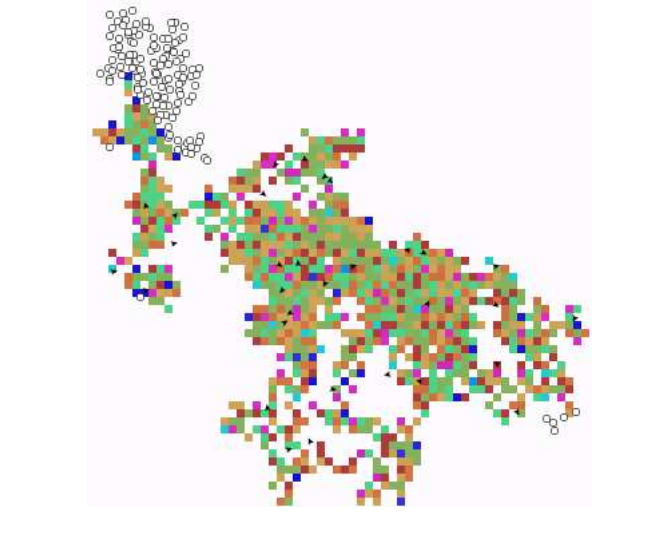
\includegraphics[scale=0.45]{pictures/Image0.png}}
\caption{Un exemple de développement de logiciel Open Source
  simulé. Les carrés sont des patches de code. Les cercles noirs
  sont des prérequis non satisfaits.}
 \end{figure}


\subsection{Données empiriques}

\subsection{Résultats}

\section{Simulation modifiée (?)}

\subsection{Modèle}

\subsection{Résultats}

\section{Comparaison des résultats}

\section{Conclusion}

\end{document}